\chapter{单一尺度下基于深度神经网络的故障诊断模型研究}
\label{cha:chapter3}

\section{引言}

在第~\ref{cha:chapter2}章中,我们使用RDFT(实数形式的傅立叶变换)将原始信号片段变换为长度与其
相等的频谱序列,并在此基础上使用平均值下采样的方法进行了特征提取,最后使用所提取的特征训练和
测试一个基于SVM的级联分类模型,达到了不错的预测精度。平均值下采样的过程是将长度为$N$的序列$X$
等分为$L$个连续的小区间,然后在各区间内计算均值,最后将这$L$个均值排成的向量作为结果。通常,
我们将$F=X/L$称为下采样的核宽度。除了平均值下采样之外,最常用的还有最大值下采样,具体的计算过
程本章会详细介绍。第~\ref{cha:chapter2}章的实验中我们也考察了使用不同核宽度的平均值下采样
进行特征提取对模型最终的预测精度的影响,我们发现随着核宽度从$2^0$到$2^7$的变化过程中,模型的
预测精度会呈现出先增高后降低的趋势。下采样实际上是用局部区域的平均或显著值来代替相应区域,从
而降低特征维度的过程。因此合适的下采样核宽度能够起到提取显著特征,缩减特征维度的作用;但是过大
的下采样核宽度会给原始特征造成破坏性,导致信息丢失严重。因此实际应用中最常见的是核宽度$F=2$的
下采样。第~\ref{cha:chapter2}章虽然在下采样核宽度$F=8$也就是$L=48$时能够获得93.81\%的预测精度,
但是分析测试集上预测结果的混淆矩阵可以发现,在个别类别的样本上表现比较差,较大的核宽度可能是
导致这种结果的原因之一。图~\ref{fig:single_pooling}是第~\ref{cha:chapter2}章中用到的单层下采样
提取特征的示意图。
\begin{figure}[ht]
  \centering%
  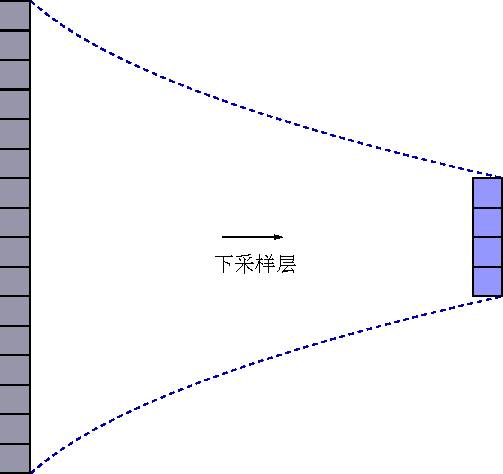
\includegraphics{single_pooling}
  \caption{单个核宽度为4的下采样}
  \label{fig:single_pooling}
\end{figure}

在卷积神经网络(Convolutional Neural Network, CNN)中,通常会有多个核宽度$F=2$的下采样操作,并
且在两个下采样操作之间往往会有至少一个卷积层。图~\ref{fig:multi_pooling}是CNN中多层下采样操作筛
选特征的示意图。使用这样的结构来处理信号频谱序列,不但可以逐层提取或筛选特征,降低特征的维度,
而且可以避免使用单个下采样操作时,核宽度过大所带来的信息丢失。
\begin{figure}[ht]
  \centering%
  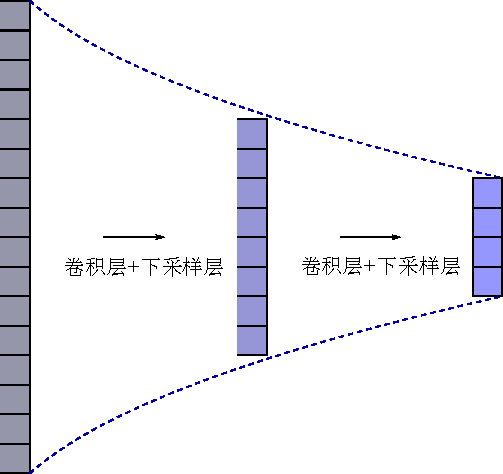
\includegraphics{multi_pooling}
  \caption{两个核宽度为2的下采样}
  \label{fig:multi_pooling}
\end{figure}

本章首先对神经网络相关的概念做了简单介绍,包括神经元的基本构成、一般神经网络的结构以及神经网络
的训练算法——反向传播算法。接下来我们介绍了卷积神经网络的结构、卷积神经网络中常用的三种层:卷积
层、下采样层和全连接层。然后我们详细介绍了本章基于卷积神经网络设计的故障诊断模型,最后在CWRU数
据集上进行实验,并且得到了比第~\ref{cha:chapter2}章更好的预测效果。

\section{基本理论}

\subsection{神经网络}
\label{subsection:nn}

\subsubsection{神经元}

在正式介绍神经网络之前,我们首先需要了解神经网络的基本组成单元——神经元。图~\ref{fig:neuron}是
一个神经元的基本结构。
\begin{figure}[ht]
  \centering%
  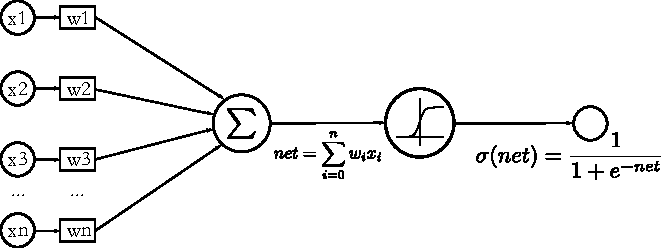
\includegraphics{neuron}
  \caption{神经元结构}
  \label{fig:neuron}
\end{figure}

假设神经元的输入记为向量$x$,相应的权重向量记为$w$,激活函数取sigmoid函数,那么神经元的输出$y$
可以通过~(\ref{equ:chap3:neuron1})式得出:
\begin{equation}
  \label{equ:chap3:neuron1}
  y = \text{sigmoid}(w^Tx)
\end{equation}

sigmoid函数的定义如~(\ref{equ:chap3:neuron2})所示。
\begin{equation}
  \label{equ:chap3:neuron2}
  \text{sigmoid}(x) = \frac{1}{1+e^{-x}}
\end{equation}

将~(\ref{equ:chap3:neuron2})代入~(\ref{equ:chap3:neuron1})可得:
\begin{equation}
  \label{equ:chap3:neuron3}
  y = \frac{1}{1+e^{-w^Tx}}
\end{equation}

sigmoid函数的图像如图~\ref{fig:sigmoid}所示。
\begin{figure}[ht]
  \centering
  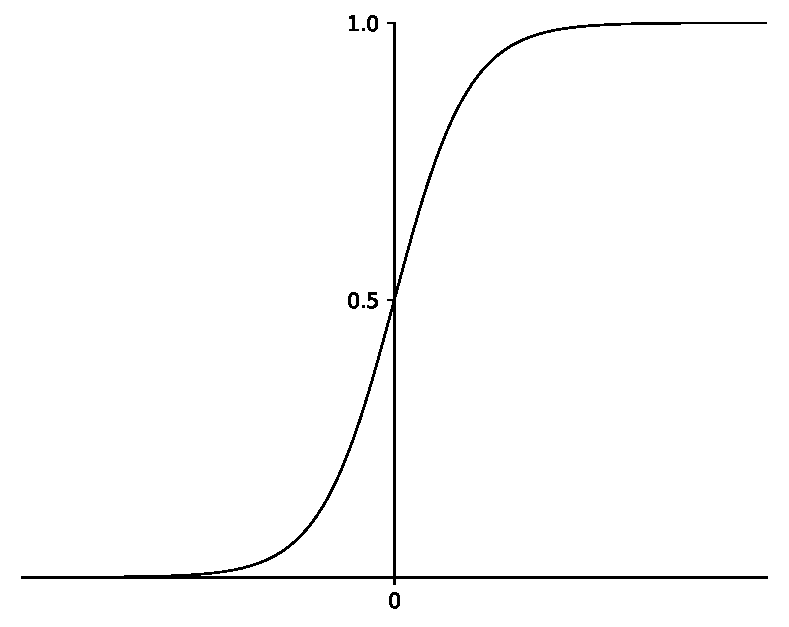
\includegraphics[height=6cm]{sigmoid}
  \caption{sigmoid函数图像}
  \label{fig:sigmoid}
\end{figure}

将sigmoid函数记作$f(x)$,那么它的导数如~(\ref{equ:chap3:derivative_sigmoid})式所示。
\begin{equation}
  \label{equ:chap3:derivative_sigmoid}
  f^\prime(x) = f(x)(1-f(x))
\end{equation}

可以看出sigmoid函数的导数可以用其自身来表示。因此,当我们得到sigmoid函数值后,就可以轻易
地计算出它的导数值。这实际上是神经网络中用到的所有激活函数的一个共同点。

\subsubsection{神经网络的结构}

神经网络实际上是大量神经元按照一定的规则连接在一起的网络结构。图~\ref{fig:fc1}是一个简单
的全连接(Fully Connected, FC)神经网络。
\begin{figure}[ht]
  \centering
  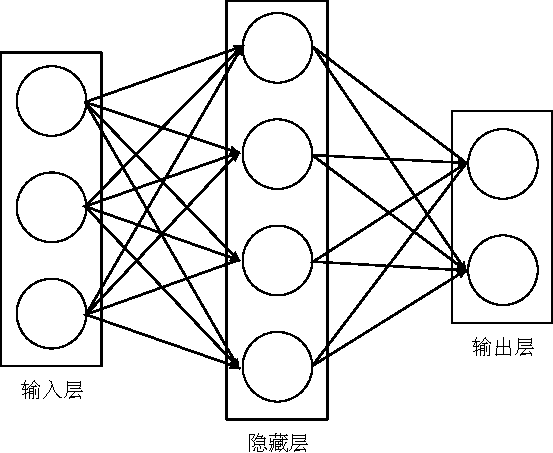
\includegraphics{fc1}
  \caption{全连接神经网络示意图}
  \label{fig:fc1}
\end{figure}

从图中可以看到,全连接神经网络分为多个层,最开始的一层称为输入层,最后面的一层称为输出层,
输入层和输出层之间的其他层称为隐藏层。同一层的神经元之间没有相互连接,相邻两层间的各神经
元之间均相互连接,这也是它被称为全连接神经网络的原因。当然神经网络还有其他很多种连接形式,
比如~\ref{subsection:cnn}节将要介绍的卷积神经网络(Convolutional Neural Network, CNN)等。

\subsubsection{神经网络的计算}

神经网络其实就是一个从输入向量到输出向量的多元非线性函数。由于神经网络是分层的,因此我们
需要从输入向量开始,使用~(\ref{equ:chap3:neuron3})式逐层向前计算,直到输出层的所有神经元计
算完毕为止。以图~\ref{fig:fc2}为例,下面简单给出神经网络的前向计算过程。
\begin{figure}[ht]
  \centering
  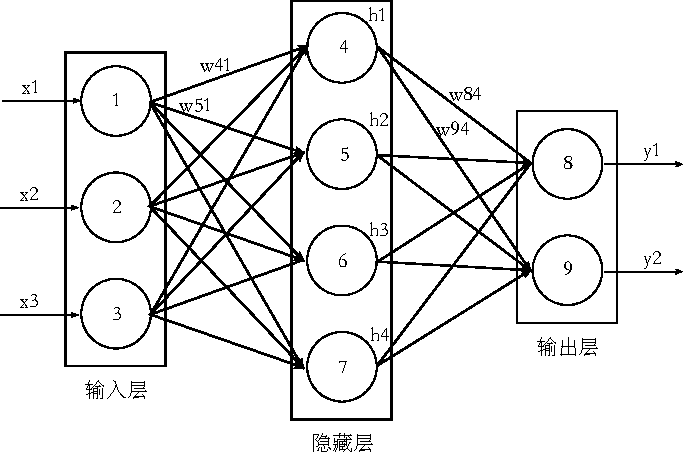
\includegraphics{fc2}
  \caption{神经网络前向计算}
  \label{fig:fc2}
\end{figure}

图中输入层的三个节点分别编号为1、2、3,隐藏层的四个节点分别编号为4、5、6、7,输出层的2个
节点分别编号为8和9。将隐藏层的四个节点处的值组成的向量记为$h=(h_1, h_2, h_3, h_4)^T$,输
入层的节点1和隐藏层的节点4之间连接的权值记为$w_{41}, w_{42}, w_{43}$,那么我们可以得到
$h_1$的计算方法如~(\ref{equ:chap3:cal_hidden})式所示。
\begin{equation}
  \label{equ:chap3:cal_hidden}
  h_1 = f(w^Tx)=f(w_{41}x_1+w_{42}x_2+w_{43}x_3+b_4)
\end{equation}

其中$f(x)$表示激活函数,$b_4$表示偏置项。按照同样的方式,我们可以计算得到$h_2$、$h_3$、
$h_4$。在得到隐藏层所有节点的值之后,我们可以计算输出层节点的值,例如节点8处的值计算方式
如~(\ref{equ:chap3:cal_output})式所示。
\begin{equation}
  \label{equ:chap3:cal_output}
  y_1 = f(w^Th)=f(w_{84}h_1+w_{85}h_2+w_{86}h_3+b_8)
\end{equation}

实际上,上面的计算过程可以写成矩阵乘法的形式,记$x=(x_1,x_2,x_3)^T$,$h=(h_1,h_2,h_3,h_4)^T$,
$y=(y_1,y_2)^T$,那么从输入层到隐藏层的计算过程可以写为:
\begin{equation}
  \label{equ:chap3:matrix_cal_hidden}
  h = f(W\cdot x)
\end{equation}

从隐藏层到输出层的计算过程可以写为:
\begin{equation}
  \label{equ:chap3:matrix_cal_output}
  y = f(W\cdot h)
\end{equation}

\subsubsection{反向传播算法}

设计好一个网络模型后,我们需要在训练样本集上通过大量的迭代计算过程来逐步学习模型的参数,也就是
各层神经元之间连接的权值$w$。神经网络的学习过程一般是通过反向传播算法(Back Propagation, BP)来
完成的。假设训练样本为$(x, d)$,其中向量$x$是训练样本的特征,向量$d$是样本的目标值。在初始化网
络的所有权值之后,首先我们使用上一节中介绍的方式计算各隐藏层的值$h$和输出层的值$y$,然后从输出
层开始,从后向前逐层计算误差项$\delta$。

对于输出层的每个节点,$\delta_i$的计算方式如~(\ref{equ:chap3:delta_i_output})式所示。
\begin{equation}
  \label{equ:chap3:delta_i_output}
  \delta_i = y_i(1-y_i)(d_i-y_i)
\end{equation}

其中,$\delta_i$是节点$i$的误差项,$y_i$是节点$i$的输出值,$d_i$是节点$i$对应的目标值。例如,
对于图~\ref{fig:fc2}中的节点8,$\delta_8$的计算方式如~(\ref{equ:chap3:delta_8})所示。
\begin{equation}
  \label{equ:chap3:delta_8}
  \delta_8 = y_1(1-y_1)(d_1-y_1)
\end{equation}

对于隐藏层中的每个节点,$\delta_i$的计算方式如~(\ref{equ:chap3:delta_i_hidden})式所示。
\begin{equation}
  \label{equ:chap3:delta_i_hidden}
  \delta_i=h_i(1-h_i)\sum_{k\in D(j)}w_{ki}\delta_k
\end{equation}

其中,$D(j)$表示与节点$j$直接相连的所有下游节点,比如在图~\ref{fig:fc2}中节点4的直接下游节点
为节点8和节点9。因此,对于节点4,$\delta_4$的计算方式如~(\ref{equ:chap3:delta_4})式所示。
\begin{equation}
  \label{equ:chap3:delta_4}
  \delta_4=h_1(1-h_1)(w_{84}\delta_8+w_{94}\delta_9)
\end{equation}

最后,我们通过~(\ref{equ:chap3:update_weights})式更新网络中的权值。
\begin{equation}
  \label{equ:chap3:update_weights}
  w_{ji} = w{ji} + \eta \delta_j x_{ji}
\end{equation}

其中,$\eta$是训练过程中设定的一个模型超参数,我们称之为学习速率。计算网络中各节点误差项
以及权值更新的公式在推导过程中本质上都是利用了复合函数的链式求导法则,具体过程本文不再赘述。

\subsection{卷积神经网络}
\label{subsection:cnn}

\subsubsection{ReLU激活函数}

通常情况下卷积神经网络中的激活函数会选择ReLU(Rectified Linear Unit)函数,而不是~\ref{subsection:nn}
中介绍的sigmoid函数,或者tanh函数。~(\ref{equ:chap3:relu})式给出了ReLU函数的定义。
\begin{equation}
  \label{equ:chap3:relu}
  f(x) = \max(0, x)
\end{equation}

图~\ref{fig:relu}给出了ReLU函数的图像。
\begin{figure}[ht]
  \centering
  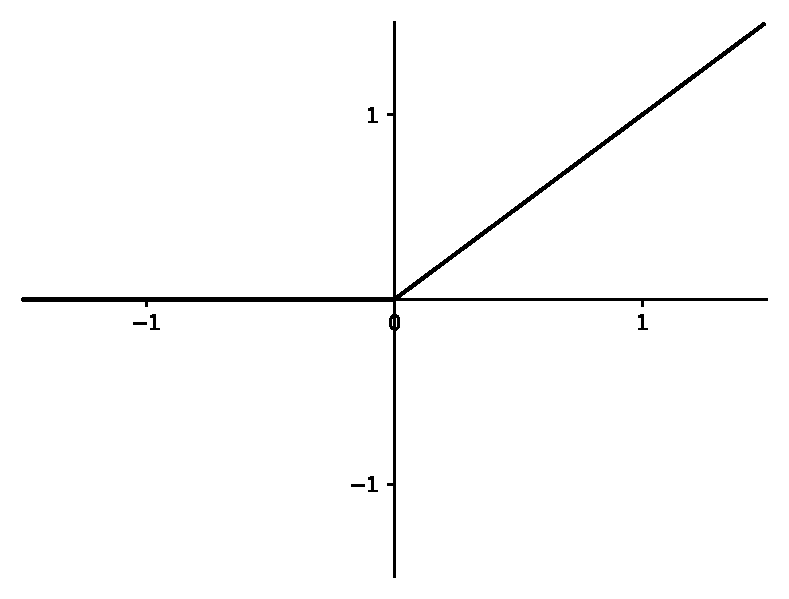
\includegraphics[height=6cm]{relu}
  \caption{ReLU激活函数的图像}
  \label{fig:relu}
\end{figure}

卷积神经网络中通常选择ReLU函数作为激活函数,是因为相对于其他的激活函数,它具有以下两个优点:

1)运算速度快。sigmoid激活函数在计算函数值时,涉及到指数和倒数运算,而ReLU激活函数只涉及到
一个比较运算,计算代价相对要小很多。

2)减轻梯度消失问题。在上一节中我们介绍了通过反向传播算法来训练神经网络,并给出了网络中权值
的更新公~(\ref{equ:chap3:update_weights})式,以及误差项的计算公~(\ref{equ:chap3:delta_i_output})式
和~(\ref{equ:chap3:delta_i_hidden})。从误差项$\delta$的计算公式可以看出,计算$\delta$的时候
总是要乘以sigmoid函数的导数值$\sigma^\prime$。从图~\ref{fig:derivative_sigmoid}中可以看出,
$\sigma^\prime$的取值范围为$(0, 1/4]$,那么从后向前逐层计算的过程中,误差项将会越来越小,
也就是梯度会越来越小,这在深层的网络结构中对于更新网络权值非常不利。而ReLU激活函数的导数值
为1,因此不会导致这个问题。
\begin{figure}[ht]
  \centering
  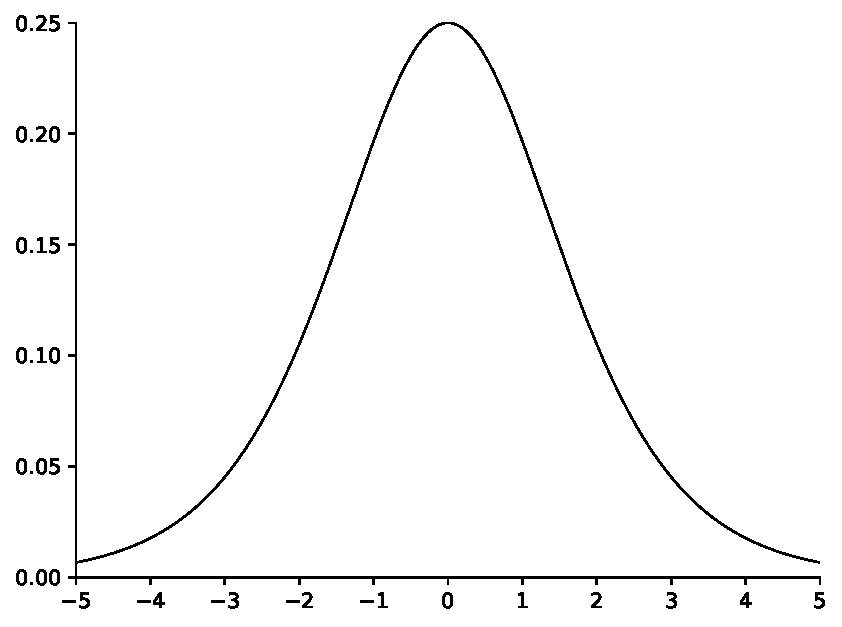
\includegraphics[height=6cm]{derivative_sigmoid}
  \caption{sigmoid导函数图像}
  \label{fig:derivative_sigmoid}
\end{figure}

\subsubsection{网络结构}

卷积神经网络和~\ref{subsection:nn}节中介绍的一般的神经网络结构非常相似。它们都是由大量带有
权值向量的神经元构成,每个神经元接受一些输入值,与权值向量做内积,然后对结果施加一个非线性
激活函数。整个网络同样有一个可导的目标函数,我们同样可以通过反向传播的方式来学习网络中的权
值。但是卷积神经网络改变了相邻两层神经元之间的连接方式,同时引入了权值共享的设定,从而极大
程度地降低了网络中权值的个数,使得网络的规模能够进一步地扩展。

首先我们来说明常规的神经网络结构在构建大规模网络时的局限。假设网络的输入是$200\times 200 
\times 3$的图像(宽度和高度均为200个像素,3个颜色通道),如果采用全联接的方式,那么第一个
隐藏层中的一个节点就会有$200\times 200\times 3=12000$个权值。当然,通常情况下每个隐藏层都
会有多个节点,而且网络中也不止有一个隐藏层,因此网络中的权值会随着网络规模的增大而急剧增加。
很明显这种全联接的网络结构会导致大量网络参数的浪费,并且很容易造成模型的过拟合。

CNN最初是针对解决图像问题而设计的,图片中的像素是排列在3个维度(宽度、高度和颜色通道)上的,
因此CNN在组建网络结构的时候仿照了图片像素的这种排列方式,即每一层的所有节点均排列为3个维度
(宽度、高度和深度)。例如对于CIFAR-10数据集中的图片,网络输入层的维度将是$32\times 32\times3$。
某一层中的节点将不再与前一层的所有节点连接,而是仅与前一层中一个较小区域中的节点连接,我们
称之为局部连接方式,本节后面部分会详细介绍。对于CIFAR-10数据集,由于这是一个10种类别的分类
问题,因此网络最后的输出层维度是$1\times 1\times 10$。图~\ref{fig:cnn}是CNN中节点排列方式
的示意图。
\begin{figure}[ht]
  \centering%
  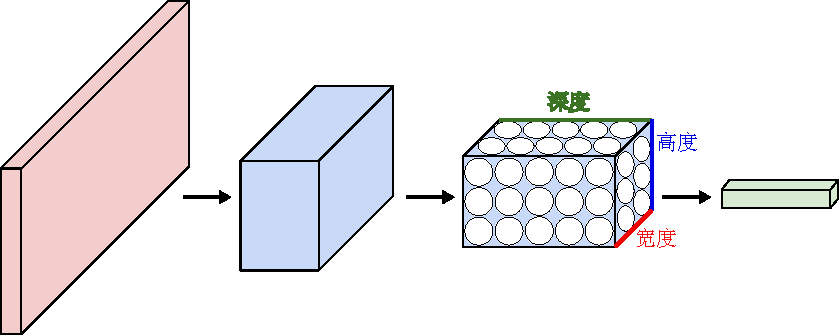
\includegraphics{cnn}
  \caption{CNN中节点排列方式示意图}
  \label{fig:cnn}
\end{figure}

从图中可以看出,一个简单的卷积神经网络由顺序排列的多个层(Layer)组成,每一层的所有节点都
排列在宽度、高度和深度3个维度上,形成一个立方体的形状,我们将排列成这种立方体形状的一层节
点称为一个特征图(Feature Map)。相邻两层特征图之间通过一个可导函数变换得到,不同的变换方
式对应着不同类型的层。最常用的一些层有:卷积层(Convolutional Layer)、下采样层(Pooling
 Layer)和全连接层(Fully Connected Layer)。我们将这些层按照一定的次序堆叠在一起就构成了
 卷积神经网络。图~\ref{fig:cnn_typical}是包含这三种层的一个典型的卷积神经网络结构。
\begin{figure}[ht]
  \centering%
  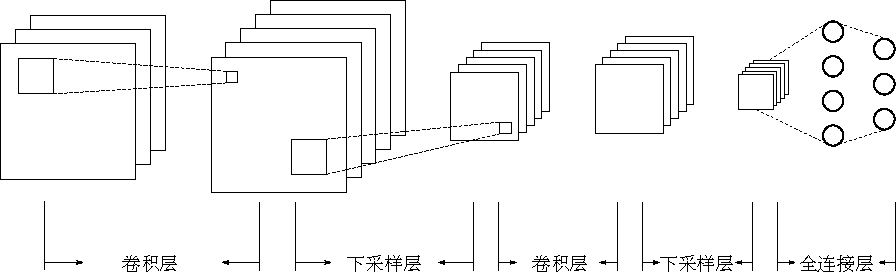
\includegraphics{cnn_typical}
  \caption{典型的CNN结构}
  \label{fig:cnn_typical}
\end{figure}

下面我们逐个介绍各个层。

1)卷积层

卷积层的参数由一组可学习的卷积核(Filter)组成。通常卷积核在空间上的尺寸(宽度和高度)比较小,
深度和上一层的深度相同。例如在图~\ref{fig:cnn_typical}中,第一个卷积层中的卷积核尺寸可以是
$5\times 5\times 3$(宽度方向和高度方向各5个像素,深度与图片通道数相等,等于3)。此外,卷积
核的个数决定了下一层特征图的深度,例如图~\ref{fig:cnn_typical}中第一个卷积层的卷积核个数为5。
各卷积核与上一层特征图沿着宽度和高度方向进行卷积运算,对运算得到的结果施加ReLU激活函数,并且
将所有卷积核对应的结果按深度方向排列在一起,即可得到下一层的特征图。图~\ref{fig:convolve}展示
了一个$3\times 3\times 3$的卷积核与$5\times 5\times 3$的特征图间的卷积运算。
\begin{figure}[ht]
  \centering%
  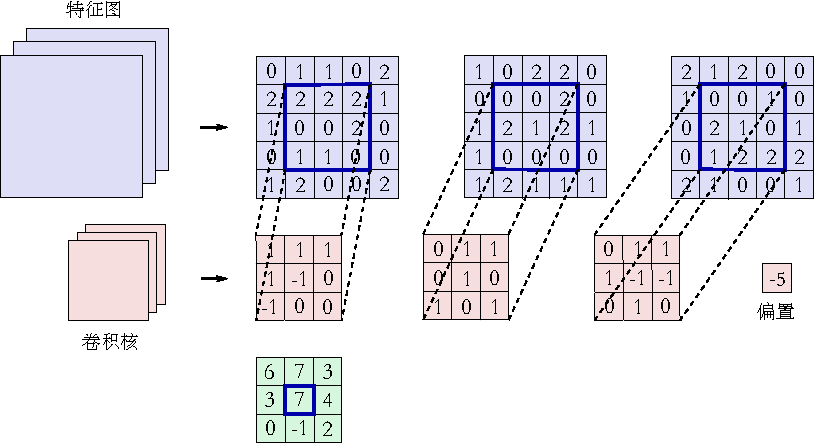
\includegraphics{convolve}
  \caption{卷积核与特征图间的卷积运算}
  \label{fig:convolve}
\end{figure}

从图中可以看出,在卷积核与特征图之间做卷积运算时,下一层特征图中的节点只和上一层中与卷积核
尺寸相同数目的节点相连接,而不是与所有节点连接,这种局部连接的方式能够在很大程度上降低网络
中权值的个数。例如对于图~\ref{fig:convolve}中的卷积运算,下一层特征图中的节点只需要与上一层
中的$3\times 3\times 3=27$个节点相连。

图~\ref{fig:convolve}展示的卷积运算过程中,步长(Stride)为1,也就是卷积核在空间方向上移动的
长度,步长也可以取其他大于1的正整数值。此外,从图中我们可以发现,经过卷积层之后,特征图在空间
上的尺寸由$5\times5$变成了$3\times 3$。很多时候,我们不希望卷积层改变特征图在空间上的尺寸,
因为这会丢失一些边缘信息。我们可以通过在边界四周补0(Zero Padding)的方式得到空间上尺寸不变的
结果,如图~\ref{fig:padding}所示。
\begin{figure}[ht]
  \centering%
  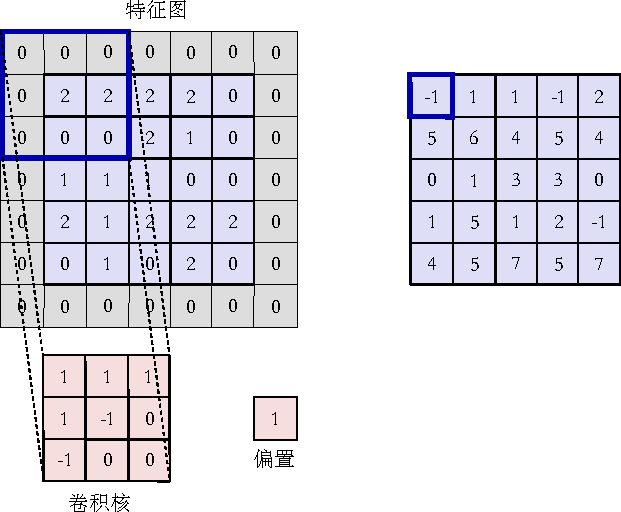
\includegraphics{padding}
  \caption{卷积过程中补零操作示意图}
  \label{fig:padding}
\end{figure}

一般地,如果卷积层输入的特征维度为$W_1\times H_1 \times D_1$,卷积核个数为$K$,卷积核在空间上
的尺寸为$F$,步长为$S$,边界四周补零的圈数为$P$,输出的特征图维度为$W_2\times H_2\times D_2$,
那么有:
\begin{equation}
  \label{equ:chap3:conv_dim}
  \left\{\begin{aligned}
    & W_2 = (W_1 - F + 2P)/S + 1 \\
    & H_2 = (H_1 - F + 2P)/S + 1 \\
    & D_2 = K
  \end{aligned}\right.
\end{equation}

因此,卷积层向网络中引入了$(F\cdot F\cdot D_1)\cdot K$个权值参数,以及$K$个偏置参数。

2)下采样层

在卷积神经网络中,通常会在连续的多个卷积层之间加入一个下采样层,它的作用在于逐步降低特征图
在空间上的尺寸,从而减少网络中的参数数量和计算量,因此能够在一定程度上防止过拟合。与卷积操作
不同,下采样层独立操作深度方向上的每一个切片,用最大值操作来对每个切片在空间上的尺寸进行压缩。
最常见的形式是核宽度为$2\times 2$、步长为2的下采样层,它可以减少75\%的特征个数。下采样层不改变
特征图的深度。图~\ref{fig:max_pooling}是最大值下采样作用于单个切片上的示意图。
\begin{figure}[ht]
  \centering%
  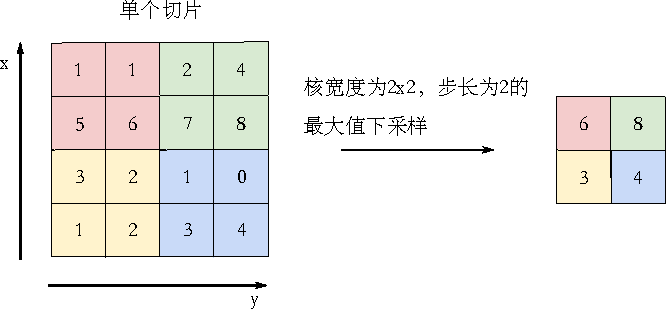
\includegraphics{max_pooling}
  \caption{单个切片上最大值下采样示意图}
  \label{fig:max_pooling}
\end{figure}

一般地,如果下采样层输入的特征图维度为$W_1\times H_1\times D_1$,核宽度为$F$,步长为$S$,输出
的特征图维度为$W_2\times H_2\times D_2$,那么有:
\begin{equation}
  \label{equ:chap3:pool_dim}
  \left\{\begin{aligned}
    & W_2 = (W_1 - F)/S + 1 \\
    & H_2 = (H_1 - F)/S + 1 \\
    & D_2 = D_1
  \end{aligned}\right.
\end{equation}

通常情况下,除了最大值下采样(Max Pooling),常见的下采样层还有平均值下采样(Average Pooling)
和L2-norm下采样。无论是哪一类下采样层,都不会向网络中引入参数。

3)全连接层

和一般的神经网络中神经元的连接方式一样,全连接层中的节点与前一层中的所有节点相连接。这一部分
在~\ref{subsection:nn}节中有详细介绍,此处不再赘述。

\section{基于卷积神经网络的故障诊断模型}

第~\ref{cha:chapter2}章中使用单层的平均值下采样对信号的频谱序列进行了特征提取,取得了不错的
效果。因此在介绍本章基于CNN的故障诊断模型之前,我们首先来验证CNN中更常用的最大值下采样从信号
的频谱序列中提取特征的效果。

同样,给定一个信号片段$x$,假设其采样点数为$N$,即$x = (x_1,x_2,...,x_N)^T$,下采样的核宽度
为$F$,下采样步长$S=F$。由~\ref{subsection:cnn}中的介绍可知,下采样之后的特征向量长度
$L = (N-F)/S+1=N/F$。与第二章中一样,我们首先对$x$做实数形式的傅立叶变换,得到$x$的RDFT频谱
序列$\widetilde{x} = (\widetilde{x}_1, \widetilde{x}_2, ..., \widetilde{x}_N)^T$。同样,为了避免样本相位的不一致对
最终模型的诊断精度产生影响,同时也避免在后续的操作中正负值相互抵消,我们对$\widetilde{x}$取了绝对
值,即$X = (|\widetilde{x}_1|, |\widetilde{x}_2|, ..., |\widetilde{x}_N|)^T$。下采样之后得到的特征向量记为
$V = (V_1, V_2, ..., V_L)^T$,那么参考平均值下采样的计算式~(\ref{equ:chap2:pooling}),最大值
下采样可以写为~(\ref{equ:chap3:max_pooling})式。
\begin{equation}
  \label{equ:chap3:max_pooling}
  V_k = \max_{j=1,...,F}X_{(k-1)F+j}, k=1,2,...,L
\end{equation}

图~\ref{fig:average_max_pooling_features}是某个采样点数为384的信号片段的原始波形、其对应的RDFT频谱序列、以及
分别使用平均值下采样和最大值下采样提取的维度为32的特征向量。
\begin{figure}[ht]
  \centering
  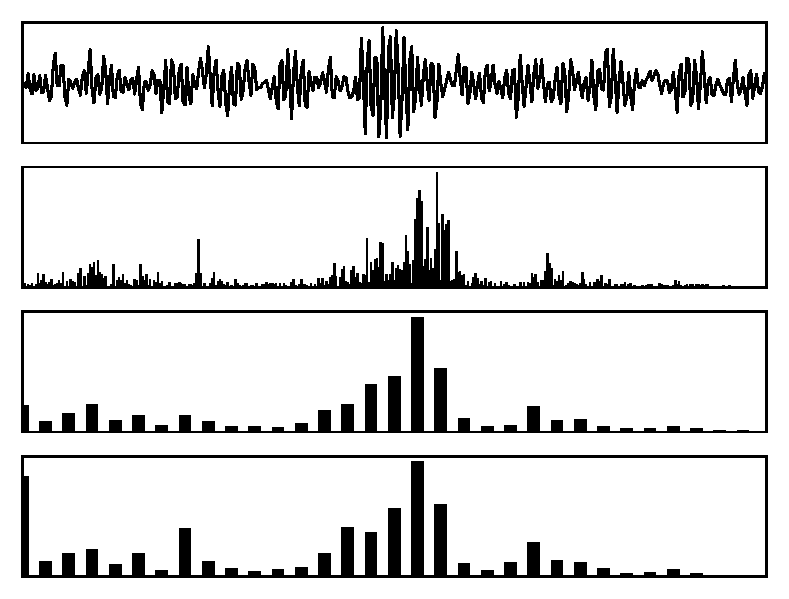
\includegraphics[height=8cm]{average_max_pooling_features}
  \caption{平均值下采样和最大值下采样提取的特征向量}
  \label{fig:average_max_pooling_features}
\end{figure}

从图中可以看出,使用最大值下采样在信号频谱上提取的特征跟使用平均值下采样获得的结果是类似的。
接下来我们用最大值下采样提取的特征训练并测试第~\ref{cha:chapter2}章中设计的故障诊断模型,在
这过程中,保持模型中的超参数设置不变,即SVM算法的惩罚因子$C=1$,高斯核宽度参数$\sigma=L$。
分别取特征个数$L$为3、6、12、24、48、96、192,对应下采样核宽度$F$为128、64、32、16、8、4、2,
依次训练并测试分类模型。与第~\ref{cha:chapter2}章中得到的结果类似,在特征个数$L=48$即下采样
核宽度$F=8$时,模型预测精度达到最高,为94.23\%。

在卷积神经网络中,我们通常会堆叠多层卷积层和下采样层,这样的结构优势在于能够逐层地提取并筛选
特征,从而得到更加高级和抽象的特征。图~\ref{fig:convnet}展示了CIFAR-10数据集上的一个CNN分类
模型的各层特征图。
\begin{figure}[ht]
  \centering%
  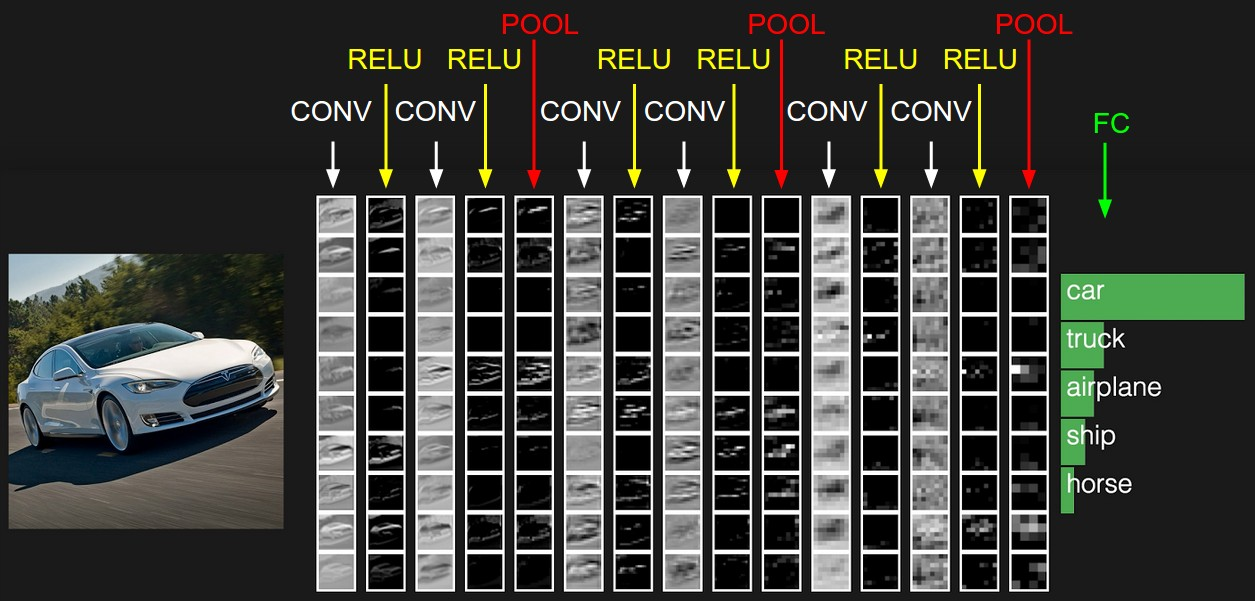
\includegraphics[width=13cm]{convnet}
  \caption{CNN模型各层特征图可视化结果示例}
  \label{fig:convnet}
\end{figure}

图~\ref{fig:convnet}中最左边是网络的输入,也就是原始图片,最右边输出对应图片的类别信息。图中
从左至右的每一列分别是网络中每一层输出的特征图。由于3维的特征图不容易显示,因此图中将特征图
沿深度方向的所有切片显示成一列。可以看出网络中最开始的几层主要是提取一些底层特征,例如图片中
的纹理、边缘、明暗等特征;网络中越后面的层提取的特征就越高级和抽象,更能反映出图片的类别信息。
因此可以说CNN网络在原始输入上提取特征的过程是逐层抽象的过程,比直接使用单层下采样提取特征的过
程显然更加合理,提取到的特征也势必更能反映类别信息。鉴于此,本章设计了一个结构与VGG类似的故障
诊断模型,如图~\ref{fig:cnn_classifier}所示。
\begin{figure}[ht]
  \centering%
  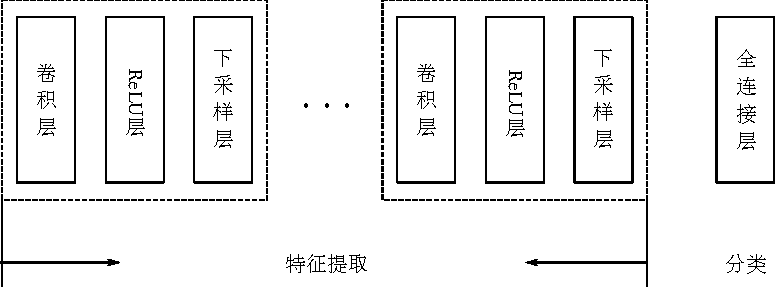
\includegraphics{cnn_classifier}
  \caption{基于CNN的故障诊断模型示意图}
  \label{fig:cnn_classifier}
\end{figure}

图~\ref{fig:cnn_classifier}中特征提取阶段基本构成单元为顺序相连的一个卷积层、一个非线性激活
层和一个下采样层,如图中虚线框所示。根据情况我们可以连续堆叠多个这样的单元来完成我们的特征提取
过程。在网络的最后,我们使用一个全连接层对提取的特征进行分类。

与第~\ref{cha:chapter2}不同,本章的特征提取和分类过程不是独立进行的,而是由同一个网络实现的。
因此,提取的特征也能够更好地反映输入数据和类别标签之间的关系。此外,特征提取环节存在大量的网络
参数可以学习,在一定程度上讲,这个模型中的特征提取方式是学习出来的,而不是直接指定的,从而能够
提取输入的信号频谱中更加本质的特征。

由于网络的输入是一维的信号频谱序列,因此我们的模型中用到的卷积层和下采样层都是沿着一维方向
进行的。图~\ref{fig:convolve_1d}是一维方向卷积操作的示例。
\begin{figure}[ht]
  \centering%
  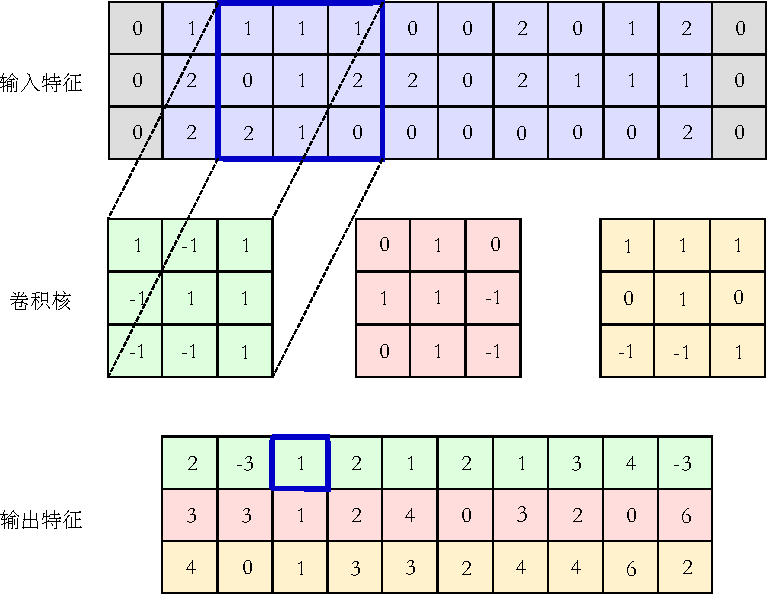
\includegraphics{convolve_1d}
  \caption{一维方向卷积操作示例}
  \label{fig:convolve_1d}
\end{figure}

图~\ref{fig:convolve_1d}中输入是维度为$3\times10$的特征图,与3个$3\times 3$的卷积核
进行一维的卷积操作后,输出维度为$3\times 10$的特征图。可以看出,一维方向的卷积操作
相当于二维情况下宽度或高度为1时的退化结果。

\section{实验验证}

\subsection{实验过程}

在本章的实验验证中,我们使用5个图~\ref{fig:cnn_classifier}中虚线框表示的基本单元顺序连接,
各层节点的数据维度变化情况如图~\ref{fig:cnn_data}所示。图中的模块1-5均表示卷积层+ReLU层
+下采样层的结构,各模块中的卷积层和下采样层的参数如表~\ref{tab:layer_parameters}所示。
\begin{figure}[ht]
  \centering%
  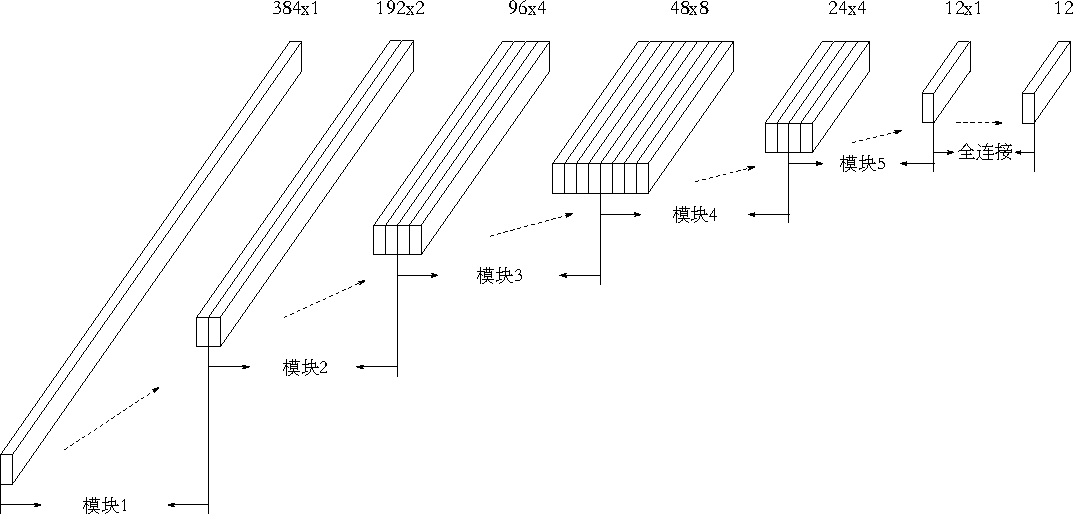
\includegraphics[width=14cm]{cnn_data}
  \caption{模型各层数据维度变化情况}
  \label{fig:cnn_data}
\end{figure}

\begin{table}[htb]
  \centering
  \begin{minipage}[t]{0.8\linewidth} % 如果想在表格中使用脚注,minipage是个不错的办法
  \caption{模型各层结构参数列表}
  \label{tab:layer_parameters}
    \begin{tabularx}{\linewidth}{lXXX}
      \toprule[1.5pt]
      网络模块 & 卷积核宽度 & 卷积核个数 & 下采样核宽度 \\\midrule[1pt]
      模块1 & 3 & 2 & 2 \\
      模块2 & 3 & 4 & 2 \\
      模块3 & 3 & 8 & 2 \\
      模块4 & 3 & 4 & 2 \\
      模块5 & 3 & 1 & 2 \\
      \bottomrule[1.5pt]
    \end{tabularx}
  \end{minipage}
\end{table}

图中网络的输入是信号片段对应的频谱序列$X$,维度为384。由于第一个模块的卷积核个数为2,
下采样核宽度为2,因此经过第一个模块后,网络中的特征图维度变为$192\times 2$;同理,经
过第二个模块后,网络中特征图的维度变为$96\times 4$;经过第三个模块后,网络中特征图的
维度变为$48\times 8$;经过第四个模块后,网络中特征图的维度变为$24\times 4$;经过第五
个模块后,网络中特征图的维度变为$12\times 1$。这个长度为12的向量就是我们的网络从原始
信号频谱序列中提取的特征向量,后面再连接一个全连接层进行故障分类。

\subsection{实验结果及分析}

网络训练好之后,我们从测试集的每一类样本中随机选择3个信号片段,分别计算其RDFT频谱序列,
并将其输入到网络中,得到网络提取的特征向量,如图~\ref{fig:cnn_features}所示。
\begin{figure}[ht]
  \centering%
  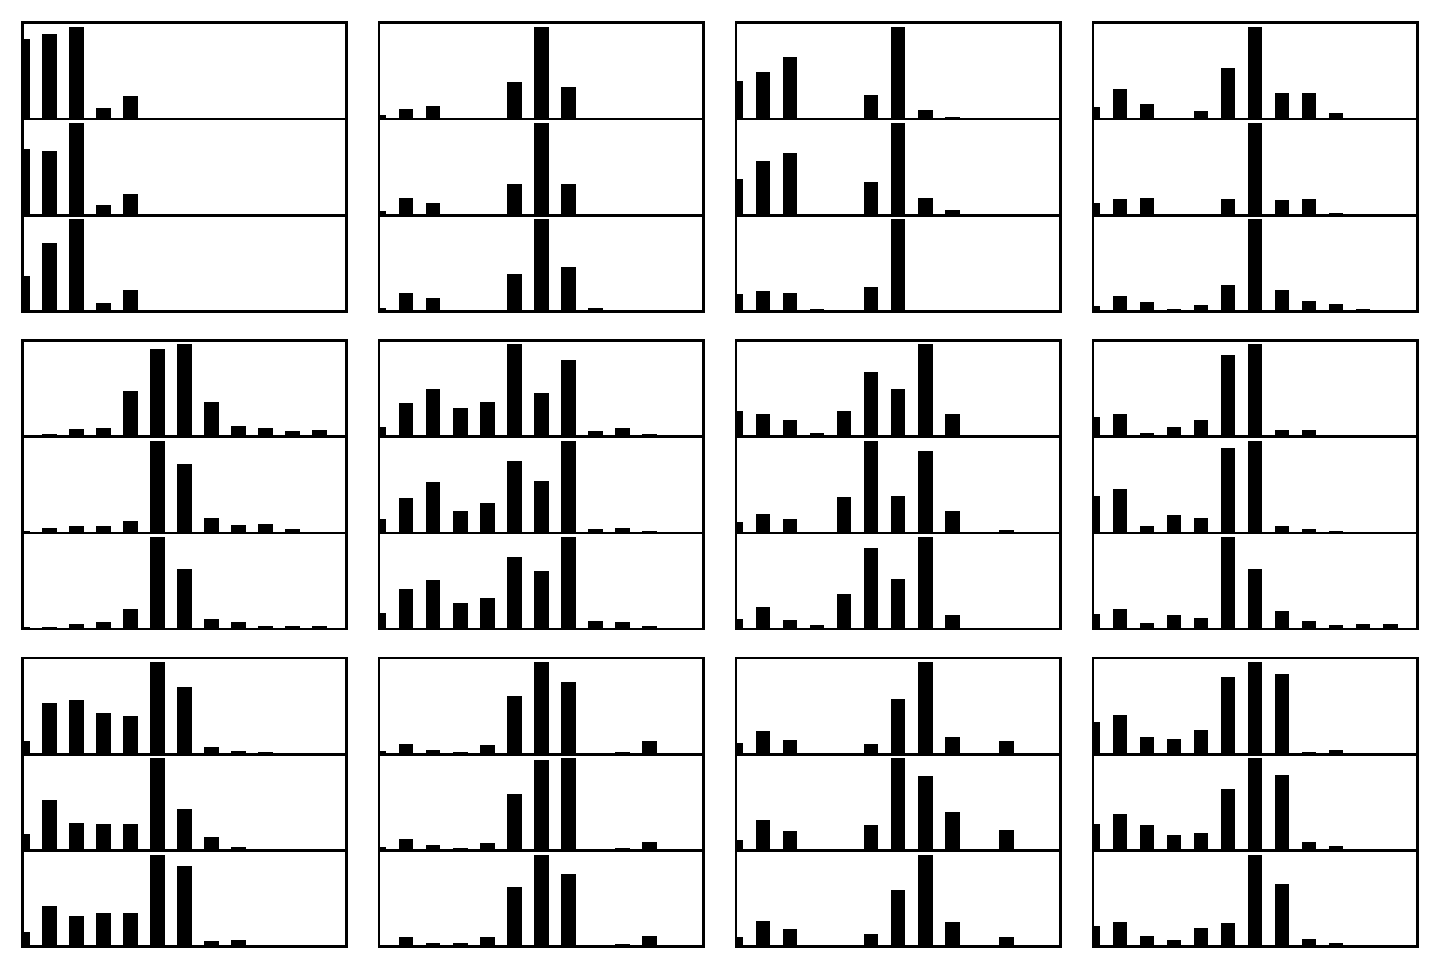
\includegraphics[height=9cm]{cnn_features}
  \caption{CNN模型提取的特征向量}
  \label{fig:cnn_features}
\end{figure}

可以看出,与图~\ref{fig:average_pooling_features_12}中显示的使用单层平均值下采样提取的
特征向量相比,使用本章中的特征提取方法获得的结果在类别之间具有更好的区分性,而同一类样
本之间的相似程度也更高。最后本章的故障诊断模型可以达到98.27\%的预测精度,也印证了这一点。
但是,本章模型的训练时间为102s,远高于第~\ref{cha:chapter2}章中基于SVM的级联分类模型训练
所用时间,这也是基于CNN的模型的缺点之一。表~\ref{tab:chap3:confusion_matrix}给出了模型在
测试集上的混淆矩阵。
\begin{table}[htb]
  \centering
  \begin{minipage}[t]{0.9\linewidth} % 如果想在表格中使用脚注,minipage是个不错的办法
  \caption{基于CNN的故障诊断模型在测试集上的混淆矩阵}
  \label{tab:chap3:confusion_matrix}
    \begin{tabularx}{\linewidth}{XXXXXXXXXXXX}
      \toprule[1.5pt]
         0 &   1 &   2 &   3 &   4 &   5 &   6 &   7 &   8 &   9 &  10 &  11 \\\midrule[1pt]
      1579 &   0 &   0 &   0 &   0 &   0 &   0 &   0 &   0 &   0 &   0 &   0 \\
         0 & 697 &   2 &  11 &   0 &   0 &   0 &   0 &   0 &   0 &   0 &   0 \\
         0 &  83 & 682 &  18 &   0 &   0 &   0 &   0 &   0 &   0 &   0 &   1 \\
         0 &  20 &   0 & 765 &   0 &   0 &   0 &   0 &   0 &   0 &   0 &   0 \\
         0 &   0 &   0 &   0 & 777 &   0 &   0 &   0 &   0 &   0 &   0 &   0 \\
         0 &   0 &   0 &   0 &   0 & 780 &   0 &   0 &   0 &   0 &   0 &   0 \\
         0 &   0 &   0 &   0 &   0 &   0 & 784 &   0 &   0 &   0 &   0 &   0 \\
         0 &   0 &   0 &   0 &   0 &   0 &   0 & 786 &   0 &   0 &   0 &   0 \\
         0 &   0 &   0 &   0 &   0 &   0 &   0 &   0 & 777 &   0 &   0 &   0 \\
         0 &   0 &   0 &   0 &   0 &   0 &   0 &   0 &   0 & 785 &   0 &   0 \\
         0 &   0 &   0 &   0 &   0 &   0 &   0 &   0 &   0 &   0 & 784 &   0 \\
         0 &   0 &   0 &   0 & 195 &   0 &   1 &   2 &   0 &  56 &   0 & 534 \\
      \bottomrule[1.5pt]
    \end{tabularx}
  \end{minipage}
\end{table}

\section{小结}

本章对神经网络做了简单的介绍,然后介绍了卷积神经网络的结构,并且基于CNN提出了一种适用
与故障诊断领域的模型,实现了对信号片段的特征提取和故障模式分类。本章设计的模型提取的
特征向量维度为12,能够在测试集上达到的预测精度为98.27\%,这与第~\ref{cha:chapter2}章
中得到的93.81\%的预测精度相比,已经有了很大的提升。此外,第~\ref{cha:chapter2}章中的
模型达到93.81\%的最佳预测精度时,提取的特征向量的维度$L=48$,特征个数相当于本章中特征
个数的4倍。从表~\ref{tab:chap2_acc_time}可以看到,当第~\ref{cha:chapter2}章中的模型取
特征维度$L=12$时,模型预测精度只能达到87.84\%。由此可见,本章中基于CNN的故障特征提取
及分类模型是非常有效的。
